\documentclass{sigchi}

% Arabic page numbers for submission. 
% Remove this line to eliminate page numbers for the camera ready copy
\pagenumbering{arabic}


% Load basic packages
\usepackage{balance}  % to better equalize the last page
\usepackage{graphics} % for EPS, load graphicx instead
\usepackage{times}    % comment if you want LaTeX's default font
\usepackage{url}      % llt: nicely formatted URLs


% llt: Define a global style for URLs, rather that the default one
\makeatletter
\def\url@leostyle{%
  \@ifundefined{selectfont}{\def\UrlFont{\sf}}{\def\UrlFont{\small\bf\ttfamily}}}
\makeatother
\urlstyle{leo}


% To make various LaTeX processors do the right thing with page size.
\def\pprw{8.5in}
\def\pprh{11in}
\special{papersize=\pprw,\pprh}
\setlength{\paperwidth}{\pprw}
\setlength{\paperheight}{\pprh}
\setlength{\pdfpagewidth}{\pprw}
\setlength{\pdfpageheight}{\pprh}

% Make sure hyperref comes last of your loaded packages, 
% to give it a fighting chance of not being over-written, 
% since its job is to redefine many LaTeX commands.
\usepackage[pdftex]{hyperref}
\hypersetup{
pdftitle={SIGCHI Conference Proceedings Format},
pdfauthor={LaTeX},
pdfkeywords={SIGCHI, proceedings, archival format},
bookmarksnumbered,
pdfstartview={FitH},
colorlinks,
citecolor=black,
filecolor=black,
linkcolor=black,
urlcolor=black,
breaklinks=true,
}

% create a shortcut to typeset table headings
\newcommand\tabhead[1]{\small\textbf{#1}}

\newcommand{\croder}{\textbf{Croder }}
\newcommand{\IDE}{\textbf{IDE }}
\newcommand{\eclipse}{\textbf{Eclipse }}


\title{Croder: Bringing the Knowledge of the Crowds into the IDE}
\author{Semih Okur \and Mihai Codoban \and Caius Brindescu \and Kyungho Lee \and Shuo Yuan}
\numberofauthors{5}
\author{
  \alignauthor Semih Okur\\
    \affaddr{University of Illinois at Urbana-Champaign}\\
    \affaddr{Urbana, IL}\\
    \email{okur2@illinois.edu}
  \alignauthor Mihai Codoban\\
    \affaddr{University of Illinois at Urbana-Champaign}\\
    \affaddr{Urbana, IL}\\
    \email{codo@illinois.edu}
  \alignauthor Caius Brindescu\\
    \affaddr{University of Illinois at Urbana-Champaign}\\
    \affaddr{Urbana, IL}\\
    \email{brind@illinois.edu}
   \alignauthor Kyungho Lee\\
    \affaddr{University of Illinois at Urbana-Champaign}\\
    \affaddr{Urbana, IL}\\
    \email{klee141@illinois.edu}
  \alignauthor Shuo Yuan\\
    \affaddr{University of Illinois at Urbana-Champaign}\\
    \affaddr{Urbana, IL}\\
    \email{syuan20@illinois.edu}
}

\begin{document}

\maketitle

\section{Introduction}
\section{Why integrate reviews into the IDE}
\section{Related work}

\section{Software development for crowds}

The main research theme that was explored throughout this project is whether software development is suitable for the crowds. \textit{Are there any software development micro-tasks which can be successfully accomplished in reasonably short time by the crowds?}

These tasks would need to take into consideration the main issue with crowdsourced tasks, that is, the lack of context. By the very nature of these short lived tasks workers cannot know the scope of the entire project. This poses severe limitations on task size since they have to be complete enough to offer the minimum amount of context for the work to be tractable, but must not be so large as to exceed the definition of micro-tasks. Deviations in any of the two conflicting constraints would make the task unattractive to workers.

We identified three activities that have a high chance of being crowdsourced.

\textbf{Code reviews}. In a usual code review, the author of the code selects a list of code snippets that he wants reviewed and then sends them to a list of reviewers. Reviewers usually consist of people working on the same project, since they have the most knowledge about the system particularities. They spend time going through the code both in isolation and together in a meeting. A list of issues is compiled at the end of the meeting. 
The usual outcomes of a code review are defect detection, design and code improvement, alternative solutions and dissemination of knowledge inside the team. 

Therefore code reviews seem to represent a natural choice for crowdsourcing since they are usually performed by a team of people and the outcome represents the accumulated knowledge of these individuals. However, in terms of review outcomes, crowdsourced code reviews would provide value only to those outcomes that do not require great context. This means that tasks such as defect detection, high level design improvements and general issues that deal with the mapping of requirements to code would not pose good candidates. 

On the other hand, crowds could be used to catch trivial and beginner mistakes. By deferring these issues, more value can be obtained from inside code reviews. Project colleagues would not waste time on these simple issues any more and could better dedicate their time and knowledge to finding high level issues that involve knowledge of the problem domain and implementation history. 

\textbf{Tests}. The crowd could be asked to write tests for different software entities such as methods or classes. Such a task could prove suitable since there are standardized, almost mechanical procedures to writing tests. For methods, the crowd could provide black box tests, by making use of the method contract, or white box tests, by making use of the method's control and data flow. For classes, the crowd would create a composition of method tests together with class contract tests. 

However, there are drawbacks and limitations to this kind of task. Tests would require some documentation of method and class contracts. The code under test may have dependencies that require to be stubbed away. High level requirement validation tests cannot be produced due to lack of context. 

\textbf{Code transformations on request}. There are a series of tedious program transformations, both refactorings and behaviour changing transformations that are tedious enough to warrant automation but require too much domain knowledge to warrant automation. On one hand, developer time would be wasted on these mechanical tasks. On the other hand, the effort required to automatize them makes it intractable to apply to many, short lived transformations. 

Examples on the refactoring side could be loop transformations for parallel execution, task boundary identification for parallel execution, code rewriting for better readability, etc. On the behaviour changing side, we can remind transformations such as introducing the visitor pattern to a large hierarchy or changing the code from using a certain library to another.

There are of course drawbacks and difficulties with this approach. Some tasks could require much more context information than the requester anticipated. The requester will have to inspect all proposed code changes which would annihilate part of the advantage of deferring work to somebody else.

From these three candidates for software development micro-tasks we chose to dedicate our efforts on providing support for code reviews. This seems like a natural starting point due to its social characteristics. From the three potential tasks, code reviews require the least amount of specialized, focused knowledge which should make them attractive to a wider audience and could potentially be of most value to the programmer. The latter justification pertains to the fact that tests and code transformations are of modest educational value to the programmer while code reviews aid in self improvement. 

\section{Crowds for software development}
One of the main challenges was finding the appropriate crowd to conduct the code review. One of the
first options was the Amazon Mechanical Turk. The main problem with this platform is the lack of
qualified workers. Code Reviewing is a very technical process that requires a large amount of knowledge.
We needed to aim for a platform where we were guaranteed to have the right audience.

Mechanical Turk tasks tend to be very simple and require only minimal knowledge and cognitive
skills. During one experiment we asked a technical question about JavaScript. Out of the 10 hits,
9 were complete in 7 days. Of those 9 tasks, only 4 useful and most of them were incomplete. This partly 
shows that the Mechanical Turk platform is ill-suited for tasks that require specialized knowledge.

Services such as eLance\footnote{\url{http://www.elance.com}} and oDesk\footnote{\url{http://www.odesk.com}}
employ a crowd to complete programming tasks. But unlike typical crowd sourcing platforms, is it
an offer based system. The requester posts the description for a task and workers bid to complete it.
The requester then chooses a winner and then work on the project can start. This system is not what
we are looking for. We needed a system where you can post your task and workers would select the
task and complete it for a predetermined amount.

StackOverflow\footnote{\url{http://www.stackoverflow.com}} allow uses to post questions and get
answers. The service is larger than most social Q\&A and technical forums. With a median answer time 
of 11 minutes and a very active user user base \cite{Mamykina2011} it makes a good candidate for a
platform to run the experiment. StackOverflow is part of a network of sites (StackExchange\footnote{\url{http://www.stackexchange.com}} that follow the same modes. One of them, \emph{Code
Review Stack Exchange}\footnote{\url{http://codereview.stackexchange.com}} is based around the
concept of concept of code review. It is this platform that we have used to test our protype.

\section{Stackexchange code review characteristics}
\section{Interface with StackExchange}

\section{Selecting code snippets}

 The first step that the programmer must undergo when composing a code review is of course choosing the code snippets that she desires to be reviewed. The programmer must be able to compose several code snippets that together paint an overall picture of the concept they want to portray. For example snippets could range from lines of code, to loops, to whole classes and packages.

 \croder allows the programmer to easily choose snippets from many places in the \IDE. The reasoning behind this is that if a resource contains or points to code, \croder should be able to transform it into a snippet. Figure \ref{fig:snippetSelection} shows  various resources which \croder can convert to code snippets, such as random editor selections, fields, methods and whole classes. As can be seen, resources originate from diverse views.

 In order to track what snippets have been added to the review so far, a view is provided that holds each snippet. Figure \ref{fig:snippetViewer} illustrates this concept.
 
 %TODO fix section reference
 With today's \croder the decision on the code snippets that are to be reviewed falls solely on the responsibility of the programmer. Section~\ref{sec:future} describes a technique which offers suggestions on other possible snippets based on the current ones.
 
\begin{figure}[hbt]
	\centering
	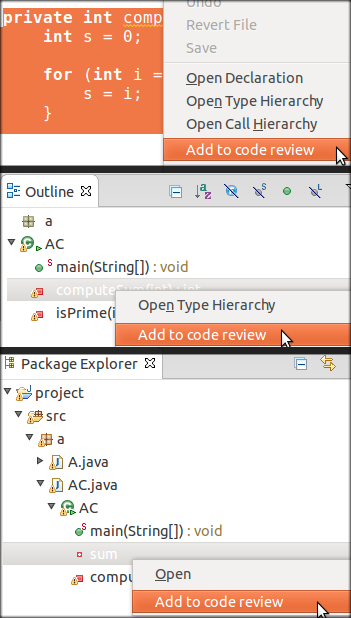
\includegraphics[scale=0.4]{snippetSelections.png}
\caption{Adding code snippets from various resources}
\label{fig:snippetSelection}
\end{figure}

\begin{figure}[hbt]
	\centering
	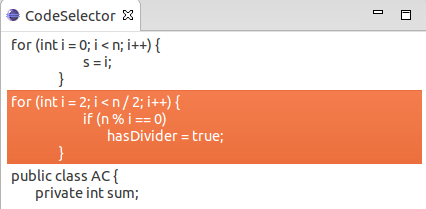
\includegraphics[scale=0.45]{snippetViewer.png}
\caption{Viewing code snippets}
\label{fig:snippetViewer}
\end{figure}

\begin{figure}[hbt]
	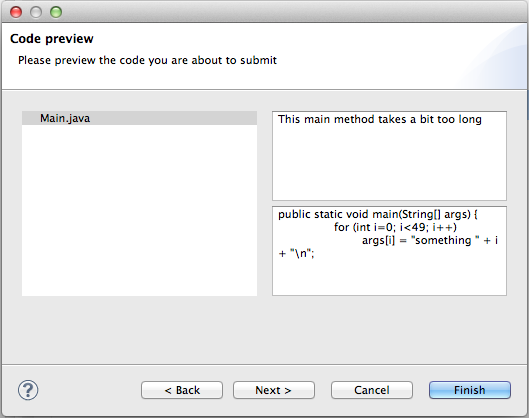
\includegraphics[width=\columnwidth]{wizard.png}
\caption{Adding comments for each snippet}
\label{fig:wizard}
\end{figure}
 
\section{Crowd sourced peer review creation}

For creating of the task we chose to implement a wizard. One of the main features is that you can ask
for \emph{structured} code review. The user can select a criteria under which code review should be
performed (performance, design, readability etc.). This helps reviews in keeping a focus on a given task.
Also, to make it easier for them to understand the code, we allow the users to add a small note regarding
the purpose and content of each code snippet. The code snippets are selected directly from the IDE.

In figure~\ref{fig:wizard} we show the design approach we took. While it is a bit crude, it does offer all
the features and presents the structured approach to creating the task. It is worth mentioning that the user
has the option to add a general comment at an earlier stage in the wizard.

\begin{figure}[hbt]
	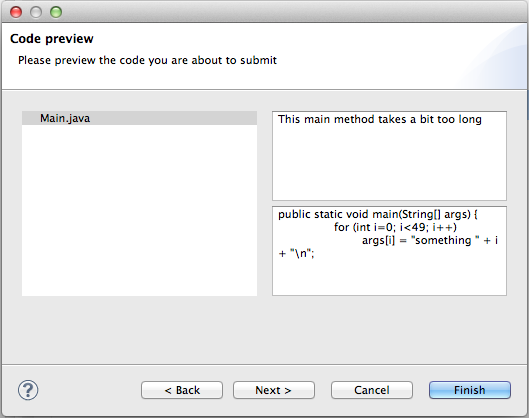
\includegraphics[width=\columnwidth]{wizard.png}
\caption{Adding comments for each snippet}
\label{fig:wizard}
\end{figure}

After entering all the details needed for a task, the user can then select the service to post it to. For the
moment we only offer integration with StackExchange, but other services can be added as well (like
oDesk, eLance etc). 

\section{Tying review outcomes to the code}

Once you submit the code, it can be difficult to remember what task relates to what code. In order to help
the programmer we decided to mark code snippets that were sent off for review. The icon on the right
rules notifies the developer if any replies have been received. 

\begin{figure}[hbt]
	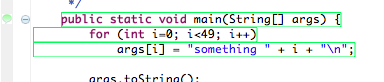
\includegraphics[width=\columnwidth]{marker.png}
\caption{The market that corresponds to the review}
\label{fig:marker}
\end{figure}

Figure~\ref{fig:marker} presents this concept. The code marked by the red box has been submitted of
review. Clicking on the marker will bring up the review task associated with it.

\section{Review management in the IDE}

In time, the programmer creates many reviews as she seeks to improve herself and her code. She may also wish to keep certain reviews for future reference. 

\croder keeps track of current and past reviews. Moreover, for each review it fetches the associated replies. Figure~\ref{fig:reviewBrowser} illustrates the Review Browser. The left pane shows the review titles while the right pane shows the replies for the currently selected review.

%TODO fix section reference
Section~\ref{sec:future} illustrates several features which can enhance the tool's capabilities via review management.

\begin{figure}[hbt]
	\centering
	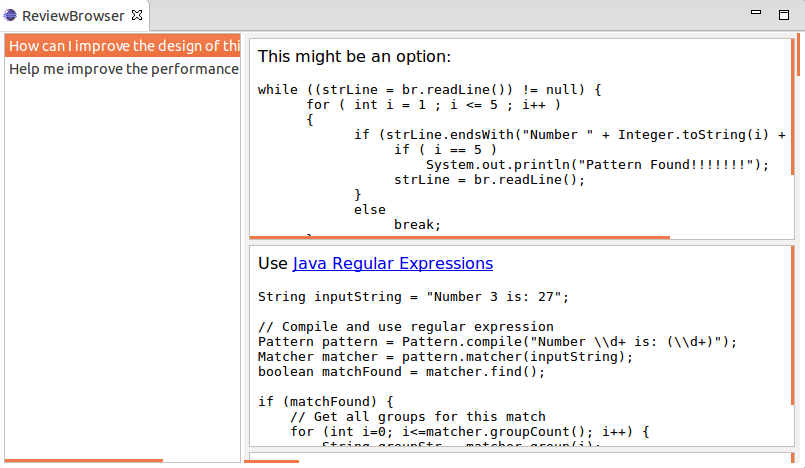
\includegraphics[scale=0.3]{reviewBrowser.png}
\caption{Viewing code snippets}
\label{fig:snippetViewer}
\end{figure}

\section{Preliminary user study}
\section{Sketches}

\section{Future Work}
\label{sec:future}

%expand bullets from presentation slides
%snippet selector
%review browser: respond, migrate to other browsers

\section{Conclusion}

\bibliographystyle{acm-sigchi}
\bibliography{paper}

\end{document}